\documentclass[11pt]{article}
\usepackage[T1]{fontenc}
\usepackage[utf8]{inputenc}
\usepackage{lmodern}
\usepackage{textcomp}
\usepackage[margin=0.9in]{geometry}
\usepackage{graphicx}
\usepackage{booktabs}
\usepackage{array}
\usepackage{amsmath,amssymb}
\usepackage[font=small,labelfont=bf]{caption}
\usepackage{microtype}
\usepackage[compact]{titlesec}
\usepackage[hidelinks]{hyperref}

\graphicspath{{../figures/}}
\newcommand{\AblBaseLowerNopunctAcc}{90.4}
\newcommand{\AblBaseLowerNopunctDrop}{2.1}
\newcommand{\AblBaseLowerNopunctTruncateSixtyfourAcc}{64.7}
\newcommand{\AblBaseLowerNopunctTruncateSixtyfourDrop}{27.8}
\newcommand{\AblBaseMaskSelfIdAcc}{92.4}
\newcommand{\AblBaseMaskSelfIdDrop}{0.1}
\newcommand{\AblBaseNormalizeTypographyAcc}{91.9}
\newcommand{\AblBaseNormalizeTypographyDrop}{0.6}
\newcommand{\AblBaseNormalizeWhitespaceAcc}{92.6}
\newcommand{\AblBaseNormalizeWhitespaceDrop}{-0.1}
\newcommand{\AblBaseStripMarkdownAcc}{92.1}
\newcommand{\AblBaseStripMarkdownDrop}{0.4}
\newcommand{\AblBaseTruncateOnetwentyeightAcc}{81.2}
\newcommand{\AblBaseTruncateOnetwentyeightDrop}{11.3}
\newcommand{\AblBaseTruncateSixtyfourAcc}{68.3}
\newcommand{\AblBaseTruncateSixtyfourDrop}{24.2}
\newcommand{\AblCnnLowerNopunctAcc}{80.9}
\newcommand{\AblCnnLowerNopunctDrop}{5.7}
\newcommand{\AblCnnLowerNopunctTruncateSixtyfourAcc}{58.0}
\newcommand{\AblCnnLowerNopunctTruncateSixtyfourDrop}{28.6}
\newcommand{\AblCnnMaskSelfIdAcc}{85.5}
\newcommand{\AblCnnMaskSelfIdDrop}{1.1}
\newcommand{\AblCnnNormalizeTypographyAcc}{87.3}
\newcommand{\AblCnnNormalizeTypographyDrop}{-0.7}
\newcommand{\AblCnnNormalizeWhitespaceAcc}{86.8}
\newcommand{\AblCnnNormalizeWhitespaceDrop}{-0.2}
\newcommand{\AblCnnStripMarkdownAcc}{87.1}
\newcommand{\AblCnnStripMarkdownDrop}{-0.5}
\newcommand{\AblCnnTruncateOnetwentyeightAcc}{75.8}
\newcommand{\AblCnnTruncateOnetwentyeightDrop}{10.8}
\newcommand{\AblCnnTruncateSixtyfourAcc}{64.4}
\newcommand{\AblCnnTruncateSixtyfourDrop}{22.3}
\newcommand{\AblLowerNopunctChanged}{100.0}
\newcommand{\AblLowerNopunctTruncateSixtyfourChanged}{100.0}
\newcommand{\AblLstmLowerNopunctAcc}{77.3}
\newcommand{\AblLstmLowerNopunctDrop}{6.0}
\newcommand{\AblLstmLowerNopunctTruncateSixtyfourAcc}{56.4}
\newcommand{\AblLstmLowerNopunctTruncateSixtyfourDrop}{26.9}
\newcommand{\AblLstmMaskSelfIdAcc}{83.4}
\newcommand{\AblLstmMaskSelfIdDrop}{-0.1}
\newcommand{\AblLstmNormalizeTypographyAcc}{82.3}
\newcommand{\AblLstmNormalizeTypographyDrop}{1.0}
\newcommand{\AblLstmNormalizeWhitespaceAcc}{83.1}
\newcommand{\AblLstmNormalizeWhitespaceDrop}{0.2}
\newcommand{\AblLstmStripMarkdownAcc}{82.6}
\newcommand{\AblLstmStripMarkdownDrop}{0.7}
\newcommand{\AblLstmTruncateOnetwentyeightAcc}{73.4}
\newcommand{\AblLstmTruncateOnetwentyeightDrop}{9.9}
\newcommand{\AblLstmTruncateSixtyfourAcc}{60.8}
\newcommand{\AblLstmTruncateSixtyfourDrop}{22.5}
\newcommand{\AblMaskSelfIdChanged}{0.8}
\newcommand{\AblNormalizeTypographyChanged}{35.7}
\newcommand{\AblNormalizeWhitespaceChanged}{0.6}
\newcommand{\AblSmallMaxAbs}{1.1}
\newcommand{\AblStripMarkdownChanged}{2.5}
\newcommand{\AblTruncateOnetwentyeightChanged}{99.1}
\newcommand{\AblTruncateSixtyfourChanged}{100.0}
\newcommand{\AvgWordLenChatGPT}{5.91}
\newcommand{\AvgWordLenClaude}{6.44}
\newcommand{\AvgWordLenDeepSeek}{6.09}
\newcommand{\AvgWordLenGemini}{5.80}
\newcommand{\AvgWordLenLlama}{5.57}
\newcommand{\AvgWordLenQwen}{6.31}
\newcommand{\BaselineAcc}{92.5}
\newcommand{\BaselineC}{100}
\newcommand{\BaselineFeatures}{400,000}
\newcommand{\BaselineFone}{92.4}
\newcommand{\BatchSize}{64}
\newcommand{\BudgetHours}{2}
\newcommand{\ChancePct}{16.7}
\newcommand{\CloseTopChatGPTPct}{8.7}
\newcommand{\CloseTopClaudePct}{1.3}
\newcommand{\CloseTopDeepSeekPct}{2.1}
\newcommand{\CloseTopGeminiPct}{2.7}
\newcommand{\CloseTopLlamaPct}{6.1}
\newcommand{\CloseTopQwenPct}{2.9}
\newcommand{\CnnBestEpoch}{6}
\newcommand{\CnnDropout}{0.3}
\newcommand{\CnnEpochsRun}{9}
\newcommand{\CnnFeatureDim}{768}
\newcommand{\CnnFilters}{256}
\newcommand{\CnnFinalTrainAcc}{93.9}
\newcommand{\CnnFinalValAcc}{87.3}
\newcommand{\CnnParams}{6,620,782}
\newcommand{\CnnSecPerEpoch}{3.4}
\newcommand{\CnnTrainSeconds}{30}
\newcommand{\CoverageMaxLen}{99.2}
\newcommand{\CoverageThreeEightFour}{86.4}
\newcommand{\CoverageTwoFiveSix}{30.0}
\newcommand{\CurlyAposChatGPT}{47.1}
\newcommand{\CurlyAposClaude}{0.1}
\newcommand{\CurlyAposDeepSeek}{52.2}
\newcommand{\CurlyAposGemini}{1.6}
\newcommand{\CurlyAposLlama}{0.0}
\newcommand{\CurlyAposQwen}{39.7}
\newcommand{\Device}{NVIDIA GeForce RTX 4060 Laptop GPU}
\newcommand{\DupAcrossModels}{0}
\newcommand{\EmDashChatGPT}{33.6}
\newcommand{\EmDashClaude}{2.8}
\newcommand{\EmDashDeepSeek}{66.2}
\newcommand{\EmDashGemini}{8.4}
\newcommand{\EmDashLlama}{0.0}
\newcommand{\EmDashQwen}{23.2}
\newcommand{\EmDashRateChatGPT}{0.28}
\newcommand{\EmDashRateClaude}{0.02}
\newcommand{\EmDashRateDeepSeek}{0.64}
\newcommand{\EmDashRateGemini}{0.08}
\newcommand{\EmDashRateLlama}{0.00}
\newcommand{\EmDashRateQwen}{0.23}
\newcommand{\EmbDim}{200}
\newcommand{\ErrBoth}{216}
\newcommand{\ErrBothSame}{144}
\newcommand{\ErrBothShareOfCnn}{60}
\newcommand{\ErrCnn}{361}
\newcommand{\ErrEither}{595}
\newcommand{\ErrLstm}{450}
\newcommand{\ErrTokensCnnCorrect}{304}
\newcommand{\ErrTokensCnnWrong}{275}
\newcommand{\ErrTokensLstmCorrect}{305}
\newcommand{\ErrTokensLstmWrong}{277}
\newcommand{\ExactStringsAllSix}{2,906}
\newcommand{\FeatCount}{38}
\newcommand{\FeatGbAcc}{79.7}
\newcommand{\FeatGbFone}{79.6}
\newcommand{\FeatLossFormatting}{0.3}
\newcommand{\FeatLossLength}{4.6}
\newcommand{\FeatLossLexical}{5.4}
\newcommand{\FeatLossPunctuation}{4.0}
\newcommand{\FeatLossTypography}{4.0}
\newcommand{\FeatLrAcc}{72.3}
\newcommand{\FeatLrFone}{72.2}
\newcommand{\FeatOnlyFormatting}{20.1}
\newcommand{\FeatOnlyLength}{59.0}
\newcommand{\FeatOnlyLexical}{55.2}
\newcommand{\FeatOnlyPunctuation}{55.5}
\newcommand{\FeatOnlyTypography}{42.4}
\newcommand{\FeatTopFive}{MATTR (window 50)}
\newcommand{\FeatTopFiveImp}{5.6}
\newcommand{\FeatTopFour}{parentheses / 100 words}
\newcommand{\FeatTopFourImp}{5.9}
\newcommand{\FeatTopOne}{type-token ratio}
\newcommand{\FeatTopOneImp}{14.1}
\newcommand{\FeatTopThree}{characters}
\newcommand{\FeatTopThreeImp}{6.8}
\newcommand{\FeatTopTwo}{curly apostrophes / 100 words}
\newcommand{\FeatTopTwoImp}{7.8}
\newcommand{\FeatWithoutFormatting}{79.4}
\newcommand{\FeatWithoutLength}{75.1}
\newcommand{\FeatWithoutLexical}{74.3}
\newcommand{\FeatWithoutPunctuation}{75.7}
\newcommand{\FeatWithoutTypography}{75.7}
\newcommand{\GradClip}{1}
\newcommand{\GroupsAllSix}{2,974}
\newcommand{\GroupsAllSixPct}{99.1}
\newcommand{\GroupsSharedBetweenSplits}{0}
\newcommand{\InputMaxLen}{32}
\newcommand{\LearningRate}{0.001}
\newcommand{\LongestModel}{Claude}
\newcommand{\LongestModelTokens}{344}
\newcommand{\LstmBestEpoch}{7}
\newcommand{\LstmDropout}{0.5}
\newcommand{\LstmEpochsRun}{10}
\newcommand{\LstmFeatureDim}{1024}
\newcommand{\LstmFinalTrainAcc}{87.7}
\newcommand{\LstmFinalValAcc}{84.3}
\newcommand{\LstmHidden}{256}
\newcommand{\LstmLayers}{2}
\newcommand{\LstmOutDim}{512}
\newcommand{\LstmParams}{8,522,094}
\newcommand{\LstmSecPerEpoch}{26.6}
\newcommand{\LstmTrainSeconds}{266}
\newcommand{\MattrChatGPT}{0.842}
\newcommand{\MattrClaude}{0.859}
\newcommand{\MattrDeepSeek}{0.878}
\newcommand{\MattrGemini}{0.828}
\newcommand{\MattrLlama}{0.765}
\newcommand{\MattrQwen}{0.869}
\newcommand{\MaxAnyFamilyPct}{0.13}
\newcommand{\MaxBoldPct}{2.0}
\newcommand{\MaxEpochs}{15}
\newcommand{\MaxLen}{512}
\newcommand{\MaxNewlinePct}{0.9}
\newcommand{\MaxOwnDeveloperPct}{0.50}
\newcommand{\MaxOwnFamilyPct}{0.07}
\newcommand{\MaxVocab}{30,000}
\newcommand{\MinFreq}{2}
\newcommand{\NoTerminalChatGPT}{1.0}
\newcommand{\NoTerminalClaude}{0.2}
\newcommand{\NoTerminalDeepSeek}{3.7}
\newcommand{\NoTerminalGemini}{1.7}
\newcommand{\NoTerminalLlama}{2.0}
\newcommand{\NoTerminalQwen}{0.7}
\newcommand{\NumSeeds}{3}
\newcommand{\OpenMaxPct}{1.7}
\newcommand{\OthersCurlyPromptsMax}{4}
\newcommand{\OthersGarbledPromptsMax}{65}
\newcommand{\OthersGarbledPromptsMin}{55}
\newcommand{\OthersUniquePromptsMax}{9}
\newcommand{\ParenRateChatGPT}{0.55}
\newcommand{\ParenRateClaude}{0.30}
\newcommand{\ParenRateDeepSeek}{2.12}
\newcommand{\ParenRateGemini}{1.36}
\newcommand{\ParenRateLlama}{0.24}
\newcommand{\ParenRateQwen}{0.69}
\newcommand{\Patience}{3}
\newcommand{\PromptGroups}{3,000}
\newcommand{\PromptInConcat}{128}
\newcommand{\PromptTokensMax}{22}
\newcommand{\PromptTokensMean}{7.8}
\newcommand{\PromptsRaw}{3,082}
\newcommand{\QtypeDefRows}{12,550}
\newcommand{\QtypeExpRows}{4,712}
\newcommand{\QtypeMixedRows}{667}
\newcommand{\QtypeOtherRows}{59}
\newcommand{\QwenCurlyPrompts}{64}
\newcommand{\QwenGarbledPrompts}{2}
\newcommand{\QwenUniquePrompts}{65}
\newcommand{\RawClasses}{22}
\newcommand{\RawRows}{66,000}
\newcommand{\RemovedDupResponses}{11}
\newcommand{\RemovedMissingEmpty}{0}
\newcommand{\RemovedRows}{12}
\newcommand{\RemovedSheetErrors}{1}
\newcommand{\RowsAllSixPct}{99.3}
\newcommand{\RqOneCnnAcc}{87.5}
\newcommand{\RqOneCnnAccStd}{0.8}
\newcommand{\RqOneCnnConfOnePct}{9.0}
\newcommand{\RqOneCnnConfOnePred}{ChatGPT}
\newcommand{\RqOneCnnConfOneTrue}{Qwen}
\newcommand{\RqOneCnnConfThreePct}{7.4}
\newcommand{\RqOneCnnConfThreePred}{DeepSeek}
\newcommand{\RqOneCnnConfThreeTrue}{Qwen}
\newcommand{\RqOneCnnConfTwoPct}{8.2}
\newcommand{\RqOneCnnConfTwoPred}{Qwen}
\newcommand{\RqOneCnnConfTwoTrue}{ChatGPT}
\newcommand{\RqOneCnnEasiest}{Claude}
\newcommand{\RqOneCnnEasiestFone}{96.6}
\newcommand{\RqOneCnnFone}{87.5}
\newcommand{\RqOneCnnFoneStd}{0.8}
\newcommand{\RqOneCnnHardest}{ChatGPT}
\newcommand{\RqOneCnnHardestFone}{80.5}
\newcommand{\RqOneCnnSecondEasiest}{Llama}
\newcommand{\RqOneCnnSecondEasiestFone}{95.4}
\newcommand{\RqOneCnnSecondHardest}{Qwen}
\newcommand{\RqOneCnnSecondHardestFone}{82.0}
\newcommand{\RqOneCnnSeedAcc}{86.6}
\newcommand{\RqOneLstmAcc}{84.6}
\newcommand{\RqOneLstmAccStd}{1.4}
\newcommand{\RqOneLstmConfOnePct}{11.8}
\newcommand{\RqOneLstmConfOnePred}{Qwen}
\newcommand{\RqOneLstmConfOneTrue}{ChatGPT}
\newcommand{\RqOneLstmConfThreePct}{8.5}
\newcommand{\RqOneLstmConfThreePred}{Qwen}
\newcommand{\RqOneLstmConfThreeTrue}{DeepSeek}
\newcommand{\RqOneLstmConfTwoPct}{10.6}
\newcommand{\RqOneLstmConfTwoPred}{Gemini}
\newcommand{\RqOneLstmConfTwoTrue}{DeepSeek}
\newcommand{\RqOneLstmEasiest}{Claude}
\newcommand{\RqOneLstmEasiestFone}{96.1}
\newcommand{\RqOneLstmFone}{84.4}
\newcommand{\RqOneLstmFoneStd}{1.6}
\newcommand{\RqOneLstmHardest}{ChatGPT}
\newcommand{\RqOneLstmHardestFone}{76.8}
\newcommand{\RqOneLstmSecondEasiest}{Llama}
\newcommand{\RqOneLstmSecondEasiestFone}{92.3}
\newcommand{\RqOneLstmSecondHardest}{Qwen}
\newcommand{\RqOneLstmSecondHardestFone}{79.4}
\newcommand{\RqOneLstmSeedAcc}{83.3}
\newcommand{\RqThreeBaseDefCross}{88.3}
\newcommand{\RqThreeBaseDefDrop}{0.7}
\newcommand{\RqThreeBaseDefIn}{89.0}
\newcommand{\RqThreeBaseExpCross}{91.0}
\newcommand{\RqThreeBaseExpDrop}{1.2}
\newcommand{\RqThreeBaseExpIn}{92.2}
\newcommand{\RqThreeBaseFullCross}{92.8}
\newcommand{\RqThreeBaseFullIn}{91.1}
\newcommand{\RqThreeCnnDefCross}{80.4}
\newcommand{\RqThreeCnnDefDrop}{1.5}
\newcommand{\RqThreeCnnDefIn}{81.8}
\newcommand{\RqThreeCnnExpCross}{83.3}
\newcommand{\RqThreeCnnExpDrop}{0.3}
\newcommand{\RqThreeCnnExpIn}{83.6}
\newcommand{\RqThreeCnnFullCross}{88.9}
\newcommand{\RqThreeCnnFullIn}{87.2}
\newcommand{\RqThreeDefTestRows}{1,981}
\newcommand{\RqThreeExpTestRows}{586}
\newcommand{\RqThreeFullTrainRows}{8,590}
\newcommand{\RqThreeLeastStable}{Gemini}
\newcommand{\RqThreeLeastStableDrop}{2.3}
\newcommand{\RqThreeLstmDefCross}{75.9}
\newcommand{\RqThreeLstmDefDrop}{0.6}
\newcommand{\RqThreeLstmDefIn}{76.4}
\newcommand{\RqThreeLstmExpCross}{80.2}
\newcommand{\RqThreeLstmExpDrop}{0.5}
\newcommand{\RqThreeLstmExpIn}{80.7}
\newcommand{\RqThreeLstmFullCross}{87.7}
\newcommand{\RqThreeLstmFullIn}{83.5}
\newcommand{\RqThreeMatchedTrainRows}{3,478}
\newcommand{\RqThreeMaxClassDrop}{5.6}
\newcommand{\RqThreeMaxClassGain}{3.9}
\newcommand{\RqThreeMaxCrossOthers}{80.2}
\newcommand{\RqThreeMaxDropAll}{1.5}
\newcommand{\RqThreeMaxDropNeural}{1.5}
\newcommand{\RqThreeMeanDropNeural}{0.7}
\newcommand{\RqThreeMinCrossClaudeLlama}{88.8}
\newcommand{\RqThreeMinDropNeural}{0.3}
\newcommand{\RqThreeMostStable}{DeepSeek}
\newcommand{\RqThreeMostStableDrop}{-0.7}
\newcommand{\RqThreeSecondLeastStable}{ChatGPT}
\newcommand{\RqThreeSecondLeastStableDrop}{1.8}
\newcommand{\RqTwoBaseBothAcc}{92.6}
\newcommand{\RqTwoBaseBothFone}{92.6}
\newcommand{\RqTwoBaseBothMinusOut}{+0.1}
\newcommand{\RqTwoBaseInAcc}{16.9}
\newcommand{\RqTwoBaseInAsciiAcc}{16.7}
\newcommand{\RqTwoBaseInAsciiFone}{13.9}
\newcommand{\RqTwoBaseInFone}{14.0}
\newcommand{\RqTwoBaseNotSharedAcc}{29.8}
\newcommand{\RqTwoBaseNotSharedQwenCorrect}{10}
\newcommand{\RqTwoBaseOutAcc}{92.5}
\newcommand{\RqTwoBaseOutFone}{92.4}
\newcommand{\RqTwoBaseSharedAcc}{16.7}
\newcommand{\RqTwoCnnBothAcc}{87.5}
\newcommand{\RqTwoCnnBothFone}{87.5}
\newcommand{\RqTwoCnnBothMinusOut}{+0.9}
\newcommand{\RqTwoCnnInAcc}{16.8}
\newcommand{\RqTwoCnnInAsciiAcc}{16.5}
\newcommand{\RqTwoCnnInAsciiFone}{10.9}
\newcommand{\RqTwoCnnInFone}{12.6}
\newcommand{\RqTwoCnnNotSharedAcc}{28.1}
\newcommand{\RqTwoCnnNotSharedQwenCorrect}{9}
\newcommand{\RqTwoCnnOutAcc}{86.6}
\newcommand{\RqTwoCnnOutFone}{86.6}
\newcommand{\RqTwoCnnSharedAcc}{16.6}
\newcommand{\RqTwoLstmBothAcc}{82.3}
\newcommand{\RqTwoLstmBothFone}{82.3}
\newcommand{\RqTwoLstmBothMinusOut}{$-$1.1}
\newcommand{\RqTwoLstmInAcc}{16.7}
\newcommand{\RqTwoLstmInAsciiAcc}{16.7}
\newcommand{\RqTwoLstmInAsciiFone}{10.4}
\newcommand{\RqTwoLstmInFone}{9.9}
\newcommand{\RqTwoLstmNotSharedAcc}{17.5}
\newcommand{\RqTwoLstmNotSharedQwenCorrect}{2}
\newcommand{\RqTwoLstmOutAcc}{83.3}
\newcommand{\RqTwoLstmOutFone}{83.0}
\newcommand{\RqTwoLstmSharedAcc}{16.7}
\newcommand{\RqTwoNotSharedN}{57}
\newcommand{\RqTwoNotSharedQwen}{10}
\newcommand{\RqTwoSharedN}{2,642}
\newcommand{\ShorterThanOneTwentyEightPct}{0.8}
\newcommand{\ShorterThanSixtyFourPct}{0.01}
\newcommand{\ShortestModel}{Llama}
\newcommand{\ShortestModelTokens}{244}
\newcommand{\SubsetRows}{17,988}
\newcommand{\SubsetRowsBefore}{18,000}
\newcommand{\TestGroups}{450}
\newcommand{\TestRows}{2,699}
\newcommand{\TimingCnnSec}{4.8}
\newcommand{\TimingLstmSec}{18.4}
\newcommand{\TokenMaxAll}{1490}
\newcommand{\TokenMedianAll}{301}
\newcommand{\TokenPNinetyNineAll}{504}
\newcommand{\TotalBaselineMinutes}{36}
\newcommand{\TotalNeuralMinutes}{79}
\newcommand{\TotalRuns}{57}
\newcommand{\TotalTrainMinutes}{115}
\newcommand{\TrainGroups}{2,100}
\newcommand{\TrainRows}{12,590}
\newcommand{\TtrChatGPT}{0.626}
\newcommand{\TtrClaude}{0.618}
\newcommand{\TtrDeepSeek}{0.678}
\newcommand{\TtrGemini}{0.616}
\newcommand{\TtrLlama}{0.531}
\newcommand{\TtrQwen}{0.702}
\newcommand{\TypesSeen}{45,213}
\newcommand{\ValGroups}{450}
\newcommand{\ValRows}{2,699}
\newcommand{\VocabSize}{30,005}
\newcommand{\WeightDecay}{0.01}
\newcommand{\WordsChatGPT}{245}
\newcommand{\WordsClaude}{298}
\newcommand{\WordsDeepSeek}{267}
\newcommand{\WordsGemini}{266}
\newcommand{\WordsLlama}{210}
\newcommand{\WordsPerSentenceChatGPT}{23.8}
\newcommand{\WordsPerSentenceClaude}{40.4}
\newcommand{\WordsPerSentenceDeepSeek}{26.8}
\newcommand{\WordsPerSentenceGemini}{34.6}
\newcommand{\WordsPerSentenceLlama}{27.5}
\newcommand{\WordsPerSentenceQwen}{22.9}
\newcommand{\WordsQwen}{219}
\newcommand{\WorstCaseMinutes}{63}



\setlength{\parskip}{2pt}
\renewcommand{\arraystretch}{1.05}
% Keep floats close to the text that refers to them and avoid half-empty float pages.
\renewcommand{\topfraction}{0.9}
\renewcommand{\bottomfraction}{0.8}
\renewcommand{\textfraction}{0.08}
\renewcommand{\floatpagefraction}{0.85}
\setcounter{topnumber}{3}
\setcounter{bottomnumber}{2}
\setcounter{totalnumber}{5}
\setlength{\textfloatsep}{9pt plus 2pt minus 2pt}
\setlength{\floatsep}{7pt plus 2pt minus 2pt}
\setlength{\intextsep}{7pt plus 2pt minus 2pt}
\setlength{\abovecaptionskip}{4pt}
\setlength{\belowcaptionskip}{3pt}

\title{\vspace{-1.2cm}Who Wrote It? Identifying LLMs from Their Responses}
\author{CMPSC 448 Course Project\\[4pt]
Team leader: Hongyu Guo\\
Team members: Hongyu Guo (individual project)}
\date{\vspace{-0.6cm}}

\begin{document}
\maketitle

\begin{abstract}
\noindent Can a classifier identify which large language model wrote a response? We study six model
families in TXD-22 using \SubsetRows{} responses and a split that keeps answers to the same prompt together.
A CNN and a bidirectional LSTM trained from scratch reach \RqOneCnnAcc\% and \RqOneLstmAcc\% test accuracy,
respectively; TF-IDF logistic regression performs best at \BaselineAcc\% (chance: \ChancePct\%).
Prompt-only classification is near chance, and adding the prompt produces no consistent improvement.
Transfer between two question forms produces small observed drops. Style features and retraining ablations
show that substantial signal survives punctuation removal and typography normalisation, although the results
are limited to this dataset and its collection process.
\end{abstract}

\section{Introduction}
Different LLMs may leave recognisable patterns in their word choice and response structure. We treat model
identification as six-way classification and investigate four questions: \textbf{RQ1}, can a CNN and an RNN
identify the model from its response? \textbf{RQ2}, does the user's prompt help? \textbf{RQ3}, does identification
transfer across question types? \textbf{RQ4}, which linguistic or structural signals distinguish the models?
Our main finding is that the responses are distinguishable within TXD-22, but a simple baseline outperforms
both neural networks. Audits and ablations help explain the signal and the limits of that finding.

\section{Problem Definition and Dataset Curation}
\label{sec:data}
\subsection{Source, labels and cleaning}
Each example is a triple (LLM name, input prompt, output response). For RQ1 the classifier receives only the
response and predicts its model-family label. We use TXD-22, released by Iqbal and Kashem on Mendeley Data
under CC BY 4.0~\cite{txd22}; we did not generate responses ourselves. According to the dataset description,
the authors sent questions spanning 30 academic and professional subjects to 17 AI systems between January
and March 2025, requesting answers of at most about 300 words. They also collected human and mixed-source
text and describe normalising Unicode and whitespace. The released CSV contains \RawRows{} rows across
\RawClasses{} classes, with columns \texttt{Question}, \texttt{Answer} and \texttt{Source}. Model versions,
generation settings and API versus chat-interface access are undocumented.

We select ChatGPT, Gemini, Claude, Llama, DeepSeek and Qwen, six model-family labels from different developers.
Human and mixed-authorship classes are excluded; restricting the study to these six also avoids labels for
products that may serve multiple underlying models. Filtering occurs before vocabulary construction or
training. The subset contains academic questions and answers, with no private information identified in
our review. We read the CSV as Windows-1252, remove one spreadsheet-error response and
\RemovedDupResponses{} exact within-model duplicates, and retain \SubsetRows{} examples. There are no
missing or empty responses and no exact response shared across model labels. Case, punctuation and symbols
are preserved because they may carry identifying information.

\begin{table}[!htb]
\centering\small
\caption{Dataset after filtering and cleaning. Words and tokens are mean counts per response; median and
P99 refer to token counts. The classes remain approximately balanced.}
\label{tab:dataset}
\begin{tabular}{lrrrrrrrrrr}
\toprule
Model & Raw & Removed & Kept & Train & Val & Test & Words & Tokens & Median & P99 \\
\midrule
ChatGPT & 3000 & 0 & 3000 & 2100 & 450 & 450 & 245 & 291 & 286 & 479 \\
Gemini & 3000 & 8 & 2992 & 2093 & 450 & 449 & 266 & 322 & 355 & 579 \\
Claude & 3000 & 0 & 3000 & 2100 & 450 & 450 & 298 & 344 & 337 & 538 \\
Llama & 3000 & 1 & 2999 & 2099 & 449 & 451 & 210 & 244 & 240 & 351 \\
DeepSeek & 3000 & 3 & 2997 & 2098 & 450 & 449 & 267 & 336 & 336 & 470 \\
Qwen & 3000 & 0 & 3000 & 2100 & 450 & 450 & 219 & 266 & 271 & 395 \\
\midrule
Total & 18000 & 12 & 17988 & 12590 & 2699 & 2699 &  &  &  &  \\
\bottomrule
\end{tabular}

\end{table}

\subsection{Audit and evaluation split}
The same questions appear across model labels: \PromptsRaw{} raw strings reduce to \PromptGroups{} groups
after normalising case, punctuation and non-ASCII characters. Of these, \GroupsAllSixPct\% have responses
from all six models. A row-level split could therefore test on questions already represented in training.
We instead assign every response to a question to the same split, using \texttt{StratifiedGroupKFold} with
20 folds: 14 for training, three for validation and three for testing. This yields a 70/15/15 split with
\TrainRows{}, \ValRows{} and \TestRows{} rows, respectively, and \GroupsSharedBetweenSplits{} shared prompt
groups. The assignment is saved and reused in every experiment. Hyperparameter and checkpoint selection
use validation data, with final scores measured on the held-out test split.

The audit revealed an encoding artefact: apostrophes in Qwen prompts can differ from the garbled characters
in the same questions under other labels. Consequently, \QwenUniquePrompts{} raw prompt strings occur
only under Qwen. Grouping on normalised text prevents those versions of the same question from crossing
splits; RQ2 separately tests whether raw prompt typography leaks the label.

Response length is a possible cue: Llama averages \ShortestModelTokens{} tokens and Claude
\LongestModelTokens{}. Self-identification is rare, with at most \MaxOwnFamilyPct\% of a model's responses
mentioning its own family. Markdown is also scarce: at most \MaxNewlinePct\% contain newlines and
\MaxBoldPct\% contain bold markup. Curly apostrophes differ substantially across models, occurring in
\CurlyAposChatGPT\% of ChatGPT and \CurlyAposDeepSeek\% of DeepSeek responses. Such typography may reflect
either generation or collection, so we test it by retraining after normalisation. Detailed audit tables
and the length-distribution plot remain available in the repository.

\section{Models and Training}
\label{sec:models}
\subsection{Representations and architectures}
The neural models use a case-sensitive word-level tokenizer that emits letter runs, digit runs, newlines
and individual punctuation or symbol characters. For example, \texttt{don't} becomes three tokens.
The vocabulary is built only from training data: tokens occurring at least \MinFreq{} times are retained
up to \MaxVocab{}, giving \VocabSize{} entries including special tokens. Unseen tokens map to an unknown
token. Responses are limited to \MaxLen{} tokens, which fully covers \CoverageMaxLen\% of training examples.
Both networks learn randomly initialised \EmbDim-dimensional embeddings without pretraining.

\paragraph{CNN.} Following Kim~\cite{kim2014}, three parallel convolutions use kernel sizes 3, 4 and 5,
with \CnnFilters{} filters each. ReLU and max-pooling over time produce a concatenated
\CnnFeatureDim-dimensional vector, followed by dropout (\CnnDropout{}) and a linear classifier with six
outputs. The model has \CnnParams{} parameters. Its filters detect local token patterns anywhere in the response.

\paragraph{BiLSTM.} The recurrent network uses a bidirectional LSTM~\cite{hochreiter1997} with
\LstmLayers{} layers and hidden size \LstmHidden{} per direction. Packed sequences skip padding. Max- and
mean-pooling over the real token outputs give a \LstmFeatureDim-dimensional vector, followed by dropout
(\LstmDropout{}) and a six-output linear layer. Embedding dropout is also applied. The model has
\LstmParams{} parameters. Pooling across time allows evidence anywhere in a response to contribute.

\subsection{Training and model selection}
Both models minimise cross-entropy using AdamW. Table~\ref{tab:training} summarises the shared settings.
Batches group similarly sized responses to reduce padding, with examples and batch order shuffled.
Python, NumPy and PyTorch seeds are fixed and cuDNN uses deterministic mode.

\begin{table}[!htb]
\centering\small
\caption{Shared neural training settings. Dropout and architecture choices are described above.}
\label{tab:training}
\begin{tabular}{ll}
\toprule
Setting & Value \\
\midrule
Learning rate / weight decay & \LearningRate{} / \WeightDecay{} \\
Batch size & \BatchSize{} \\
LSTM gradient clipping & Norm \GradClip{} \\
Checkpoint selection & Highest validation macro-F1 \\
Early stopping & \Patience{} epochs without improvement \\
Maximum training length & \MaxEpochs{} epochs \\
\bottomrule
\end{tabular}
\end{table}

A validation-only grid with seed 42 tests CNN filters \{128, 256\} and dropout \{0.3, 0.5\}, and BiLSTM
hidden sizes \{128, 256\} and layer counts \{1, 2\}. The selected architectures are those described above
and are reused in later experiments. The full grid is saved in \texttt{results/tuning/}.
RQ1 averages \NumSeeds{} seeds; RQ2--RQ4 use seed 42. We report accuracy and macro-F1, with per-class F1
and confusion matrices to show differences between labels. Reported standard deviations describe
seed variability, not confidence intervals. All \TotalRuns{} training runs took \TotalTrainMinutes{}
minutes on a \Device{}.

\paragraph{TF-IDF reference.} Logistic regression uses case-sensitive word 1--2-grams and character
2--5-grams, sublinear term frequency and \BaselineFeatures{} features. Its regularisation strength
($C=\BaselineC$) is selected on validation data. This baseline tests whether frequency-based features
are sufficient without learning a neural representation.

\section{Results}
\subsection{RQ1: identifying the model from its response}
Table~\ref{tab:rq1} shows that both networks substantially exceed chance on held-out prompt groups.
The CNN achieves \RqOneCnnAcc{} $\pm$ \RqOneCnnAccStd\% accuracy and the BiLSTM
\RqOneLstmAcc{} $\pm$ \RqOneLstmAccStd\%. The CNN has a higher average score and trains faster:
the seed-42 runs take \CnnTrainSeconds{} and \LstmTrainSeconds{} seconds, respectively.
With only \NumSeeds{} seeds, the architectural comparison remains limited.

\begin{table}[!htb]
\centering\small
\caption{RQ1 on \TestRows{} test responses. Neural results are mean $\pm$ standard deviation over
\NumSeeds{} seeds. The final six columns are per-class F1 (\%).}
\label{tab:rq1}
\begin{tabular}{lccrrrrrr}
\toprule
Model & Accuracy & Macro-F1 & ChatGPT & Gemini & Claude & Llama & DeepSeek & Qwen \\
\midrule
CNN & 87.5 $\pm$ 0.8 & 87.5 $\pm$ 0.8 & 80.5 & 88.0 & 96.6 & 95.4 & 82.4 & 82.0 \\
BiLSTM & 84.6 $\pm$ 1.4 & 84.4 $\pm$ 1.6 & 76.8 & 82.2 & 96.1 & 92.3 & 79.7 & 79.4 \\
\midrule
TF-IDF + LR & 92.5 & 92.4 & 88.2 & 92.8 & 98.0 & 98.9 & 89.2 & 87.4 \\
Chance & 16.7 & -- & -- & -- & -- & -- & -- & -- \\
\bottomrule
\end{tabular}

\end{table}

TF-IDF logistic regression performs best at \BaselineAcc\%. A plausible explanation is that the networks
must learn millions of parameters from \TrainRows{} training examples, while the baseline directly
represents recurring word and character patterns. The CNN's training accuracy is \CnnFinalTrainAcc\%
at its selected epoch versus \CnnFinalValAcc\% on validation, consistent with overfitting. Training curves
are available in \texttt{figures/training\_curves.pdf}. These observations help explain the baseline's
advantage but do not establish a single cause.

Claude and Llama are easiest to recognise: CNN F1 is \RqOneCnnEasiestFone\% and
\RqOneCnnSecondEasiestFone\%, respectively. ChatGPT and Qwen are harder, at
\RqOneCnnHardestFone\% and \RqOneCnnSecondHardestFone\%. Figure~\ref{fig:confusion} shows that these
labels are confused in both directions. Claude's long sentences and Llama's shorter, less diverse responses
provide possible explanations for their distinctive profiles; RQ4 examines these characteristics.

\begin{figure}[!htb]
\centering
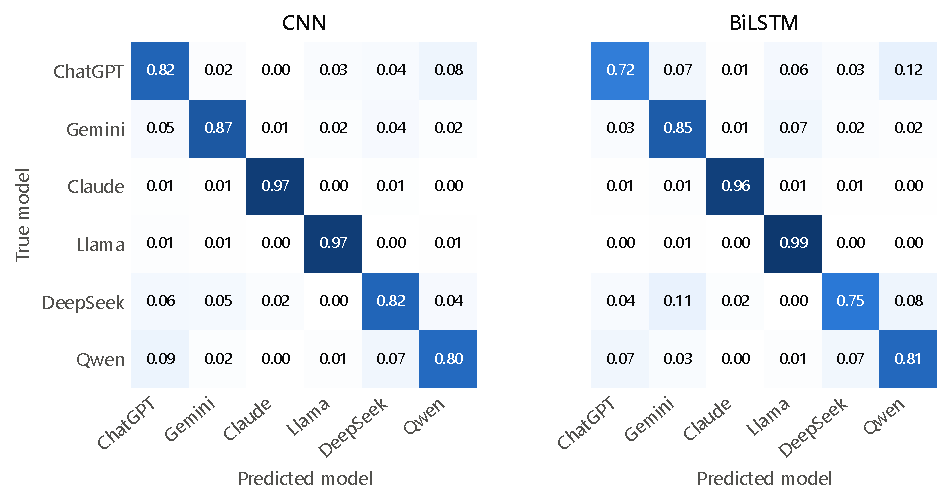
\includegraphics[width=0.85\linewidth]{confusion_rq1.pdf}
\caption{RQ1 confusion matrices averaged over \NumSeeds{} seeds. Rows are true labels, columns are
predictions, and each row sums to one. The diagonal gives per-class recall.}
\label{fig:confusion}
\end{figure}

\subsection{RQ2: does the prompt help?}
We compare prompt-only, response-only and combined inputs. Combined inputs concatenate
\texttt{[INP] prompt [OUT] response}, allowing \PromptInConcat{} prompt tokens and \MaxLen{} response
tokens; the longest prompt has only \PromptTokensMax{} tokens. All comparisons in
Table~\ref{tab:rq2} use seed 42. Thus its response-only scores (CNN \RqOneCnnSeedAcc\%, BiLSTM
\RqOneLstmSeedAcc\%) differ from the multi-seed means in RQ1.

\begin{table}[!htb]
\centering\small
\caption{RQ2 test accuracy and macro-F1 (\%), seed 42. ``ASCII'' removes non-ASCII characters and
apostrophes from prompts before retraining. Chance refers to accuracy.}
\label{tab:rq2}
\begin{tabular}{lcccccccc}
\toprule
 & \multicolumn{2}{c}{Input only} & \multicolumn{2}{c}{Input only (ASCII)} & \multicolumn{2}{c}{Output only} & \multicolumn{2}{c}{Input + output} \\
\cmidrule(lr){2-3}\cmidrule(lr){4-5}\cmidrule(lr){6-7}\cmidrule(lr){8-9}
Model & Acc. & F1 & Acc. & F1 & Acc. & F1 & Acc. & F1 \\
\midrule
CNN & 16.8 & 12.6 & 16.5 & 10.9 & 86.6 & 86.6 & 87.5 & 87.5 \\
BiLSTM & 16.7 & 9.9 & 16.7 & 10.4 & 83.3 & 83.0 & 82.3 & 82.3 \\
TF-IDF + LR & 16.9 & 14.0 & 16.7 & 13.9 & 92.5 & 92.4 & 92.6 & 92.6 \\
\midrule
Chance & 16.7 & -- & 16.7 & -- & 16.7 & -- & 16.7 & -- \\
\bottomrule
\end{tabular}

\end{table}

\paragraph{Prompt-only prediction.} Accuracy is near \ChancePct\%, as expected when the same question
appears under all six labels. Small deviations arise from incomplete groups and prompt encoding differences.
Among \RqTwoNotSharedN{} test rows whose raw prompt is not shared by all six models, the baseline correctly
identifies all \RqTwoNotSharedQwen{} Qwen rows and the CNN identifies
\RqTwoCnnNotSharedQwenCorrect{}. Removing the encoding cue yields prompt-only accuracies of
\RqTwoCnnInAsciiAcc\%, \RqTwoLstmInAsciiAcc\% and \RqTwoBaseInAsciiAcc\%. Prompt-only success can therefore
reflect dataset assembly rather than a property of the generating model.

\paragraph{Adding the prompt.} Compared with response-only input, accuracy changes by
\RqTwoCnnBothMinusOut{} points for the CNN, \RqTwoLstmBothMinusOut{} for the BiLSTM and
\RqTwoBaseBothMinusOut{} for TF-IDF. These runs show no consistent benefit. Because they use one seed,
small differences should be interpreted cautiously; they do not establish that prompt context could never
help under a different dataset design.

\section{In-Depth Analyses}
\subsection{RQ3: transfer across question types}
TXD-22 has no task labels or clear coding, calculation and creative-writing subsets. We therefore test
a narrower shift: \emph{definitional} prompts beginning with words such as ``what'' or ``define'', versus
\emph{explanatory} prompts beginning with ``explain'', ``how'' or ``why''. Definitional openings that also
contain explanatory terms are labelled mixed and excluded, along with other unmatched prompts.
Rules are in \texttt{src/prepare.py}; a spot-check of ten prompts per type confirmed the intended rule
assignments, although some definitional questions ask for more than a definition.

We train in both directions. Definitional training groups are subsampled to match the explanatory group
count, giving about \RqThreeMatchedTrainRows{} rows per training set. Early stopping uses only source-type
validation rows. For each target test set, we compare same-type and other-type training on the same rows
(Table~\ref{tab:rq3}). Architecture settings are inherited from RQ1 rather than independently retuned for
transfer, so this is not a completely target-independent model-selection protocol.

\begin{table}[!htb]
\centering\small
\caption{RQ3, seed 42. ``In'' means same-type training and ``Cross'' means size-matched other-type training.
Drops are percentage-point differences; F1 is macro-F1.}
\label{tab:rq3}
\begin{tabular}{llrrrrrrr}
\toprule
Model & Test question type & $n$ & In acc. & Cross acc. & Drop & In F1 & Cross F1 & Drop \\
\midrule
CNN & Definitional & 1981 & 81.8 & 80.4 & +1.5 & 81.7 & 80.3 & +1.4 \\
CNN & Explanatory & 586 & 83.6 & 83.3 & +0.3 & 83.6 & 83.3 & +0.3 \\
\midrule
BiLSTM & Definitional & 1981 & 76.4 & 75.9 & +0.6 & 76.3 & 75.7 & +0.5 \\
BiLSTM & Explanatory & 586 & 80.7 & 80.2 & +0.5 & 80.7 & 80.5 & +0.2 \\
\midrule
TF-IDF + LR & Definitional & 1981 & 89.0 & 88.3 & +0.7 & 88.9 & 88.2 & +0.7 \\
TF-IDF + LR & Explanatory & 586 & 92.2 & 91.0 & +1.2 & 92.1 & 90.9 & +1.2 \\
\bottomrule
\end{tabular}

\end{table}

The neural accuracy drops range from \RqThreeMinDropNeural{} to \RqThreeMaxDropNeural{} points.
Claude and Llama remain the most identifiable labels, with cross-type F1 at least
\RqThreeMinCrossClaudeLlama\% across the four neural settings. These are small observed drops under a
limited question-form shift, not evidence of generalisation to substantially different tasks. One seed
cannot establish equivalence or rule out a meaningful transfer loss. Both types still concern academic
subjects and share the same collection instructions. Training-set size also matters: using all
\RqThreeFullTrainRows{} definitional rows raises CNN accuracy on explanatory questions from
\RqThreeCnnExpCross\% to \RqThreeCnnFullCross\%. Detailed per-class changes are saved in
\texttt{results/rq3/transfer.csv}.

\subsection{RQ4: characteristics and retraining ablations}
\label{sec:stylometry}
We compute \FeatCount{} features in five groups: length, lexical diversity and related statistics,
punctuation, typography, and formatting. Moving-average type-token ratio (MATTR) uses a fixed 50-word
window to reduce the length dependence of ordinary type-token ratio~\cite{covington2010}.
Logistic regression using these features reaches \FeatLrAcc\% accuracy; histogram gradient boosting
reaches \FeatGbAcc\%. Thus aggregate response statistics carry substantial identifying information.

\begin{figure}[!htb]
\centering
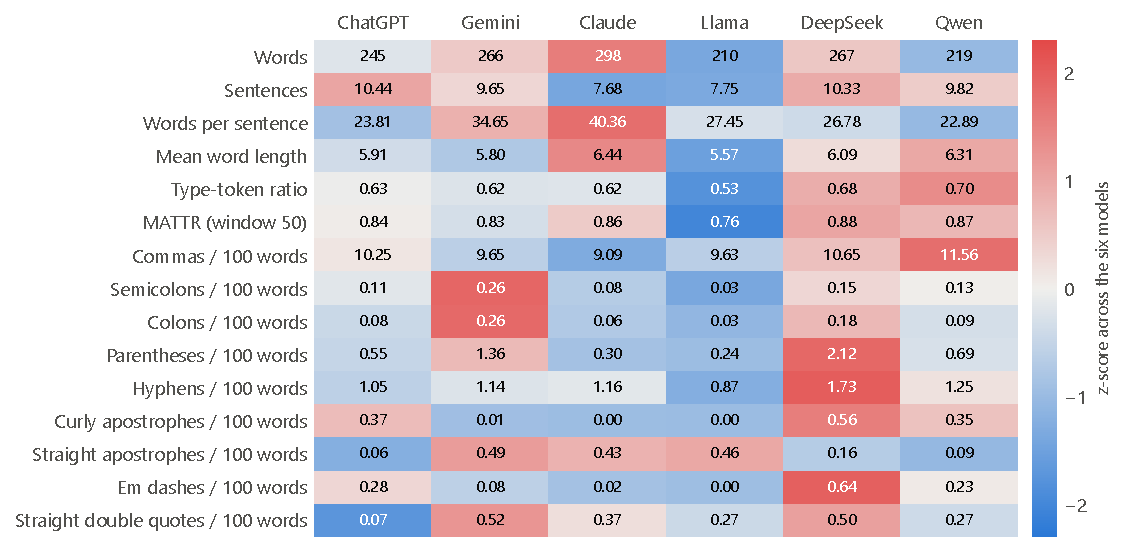
\includegraphics[width=0.74\linewidth]{rq4_feature_profiles.pdf}
\caption{Selected stylometric means by model. Cell values are means; colour gives the z-score of each
feature's mean across the six labels. These descriptive differences do not by themselves establish
what a neural classifier uses.}
\label{fig:profiles}
\end{figure}

Claude averages \WordsPerSentenceClaude{} words per sentence, compared with \WordsPerSentenceQwen{}
for Qwen. Llama has lower MATTR (\MattrLlama{}) than DeepSeek (\MattrDeepSeek{}), and DeepSeek uses
more parentheses. Feature-group classifiers reach \FeatOnlyLength\% using length alone,
\FeatOnlyLexical\% using lexical statistics, \FeatOnlyPunctuation\% using punctuation and
\FeatOnlyTypography\% using typography. Removing length from the full feature classifier lowers accuracy
by \FeatLossLength{} points, suggesting overlapping cues. This does not quantify length's contribution
to the neural models.

Training-split n-grams ranked by log-odds with a Dirichlet prior~\cite{monroe2008} provide examples:
Claude favours connecting words such as ``while'' and ``including'', DeepSeek favours parentheses and
``e.g.'', and Qwen favours ``for example''. Shared prompts reduce topic confounding, but responses may
still select different content, so these are descriptive associations rather than pure measures of style.
The full n-gram rankings and feature-group results remain in \texttt{results/rq4/}.

\paragraph{Ablation design.} We apply each transformation to training, validation and test responses,
retrain from scratch, and compare with the unmodified seed-42 model. Transformations remove markdown,
normalise whitespace, lowercase and remove punctuation, truncate text, mask model/developer names, or
normalise typography. Table~\ref{tab:ablations} reports all conditions. The common seed makes runs easier
to compare, but single-seed differences have no experiment-specific uncertainty estimate.

\begin{table}[!htb]
\centering\small
\caption{RQ4 retraining ablations, seed 42. Accuracy is in percent; $\Delta$ is the change from the
unmodified seed-42 model in percentage points.}
\label{tab:ablations}
\begin{tabular}{lrrrrrrr}
\toprule
 & Responses & \multicolumn{2}{c}{CNN} & \multicolumn{2}{c}{BiLSTM} & \multicolumn{2}{c}{TF-IDF + LR} \\
\cmidrule(lr){3-4}\cmidrule(lr){5-6}\cmidrule(lr){7-8}
Responses modified & changed (\%) & Acc. & $\Delta$ & Acc. & $\Delta$ & Acc. & $\Delta$ \\
\midrule
Original text & -- & 86.6 & -- & 83.3 & -- & 92.5 & -- \\
\midrule
(a) Markdown stripped & 2.5 & 87.1 & +0.5 & 82.6 & $-$0.7 & 92.1 & $-$0.4 \\
(b) Whitespace normalised & 0.6 & 86.8 & +0.2 & 83.1 & $-$0.2 & 92.6 & +0.1 \\
(c) Lowercase, no punctuation & 100.0 & 80.9 & $-$5.7 & 77.3 & $-$6.0 & 90.4 & $-$2.1 \\
(d) First 128 tokens & 99.1 & 75.8 & $-$10.8 & 73.4 & $-$9.9 & 81.2 & $-$11.3 \\
(d) First 64 tokens & 100.0 & 64.4 & $-$22.3 & 60.8 & $-$22.5 & 68.3 & $-$24.2 \\
(e) Model names masked & 0.8 & 85.5 & $-$1.1 & 83.4 & +0.1 & 92.4 & $-$0.1 \\
(f) Typography normalised & 35.7 & 87.3 & +0.7 & 82.3 & $-$1.0 & 91.9 & $-$0.6 \\
(c)+(d) Words only, first 64 & 100.0 & 58.0 & $-$28.6 & 56.4 & $-$26.9 & 64.7 & $-$27.8 \\
\bottomrule
\end{tabular}

\end{table}

\paragraph{Formatting and typography.} Markdown removal, whitespace normalisation and name masking
alter only \AblStripMarkdownChanged\%, \AblNormalizeWhitespaceChanged\% and \AblMaskSelfIdChanged\%
of responses, respectively, and change accuracy little. Their limited effect is consistent with the audit.
Typography normalisation alters \AblNormalizeTypographyChanged\% of responses but also leaves scores
close to the originals. This suggests that the tested typographic distinctions are not necessary for high
accuracy after retraining, even though they are informative alone. It does not exclude other collection
artefacts or prove that the original classifier ignored typography.

\paragraph{Punctuation and amount of text.} Lowercasing and punctuation removal reduce CNN accuracy
from \RqOneCnnSeedAcc\% to \AblCnnLowerNopunctAcc\% and BiLSTM accuracy from \RqOneLstmSeedAcc\%
to \AblLstmLowerNopunctAcc\%. Substantial signal survives, but this condition retains length and word
order and does not isolate lexical information. Truncation produces larger drops: the CNN reaches
\AblCnnTruncateOnetwentyeightAcc\% with 128 tokens and \AblCnnTruncateSixtyfourAcc\% with 64.
It removes both response-length information and much of the available text; these effects cannot be separated
here. The combined lowercase/no-punctuation, first-64-token condition still reaches
\AblCnnLowerNopunctTruncateSixtyfourAcc\%, above chance. Together, these results support contributions
from word patterns and structure without assigning a precise share to each.

\subsection{Error analysis}
The seed-42 CNN makes \ErrCnn{} errors and the BiLSTM \ErrLstm{} on \TestRows{} responses;
\ErrBoth{} errors are shared. CNN errors are shorter on average than correct predictions
(\ErrTokensCnnWrong{} versus \ErrTokensCnnCorrect{} tokens), consistent with less text providing less
evidence, though this association is not causal proof.
Two examples, selected as the first test row for their shared confusion pair, illustrate ambiguous responses.
Both networks label a Qwen answer about tries as DeepSeek; its opening, ``A trie (pronounced `try')'',
contains a parenthetical aside associated with DeepSeek in the feature analysis. Both also label a ChatGPT
answer about sockets as Qwen; the opening is a generic definition. These examples suggest possible explanations,
but examining an opening alone cannot establish why the networks made the prediction. Complete examples
and error summaries are saved in \texttt{results/rq1/}.

\section{Lessons, Limitations and Next Steps}
\paragraph{Lessons and experience.} The data audit changed the evaluation design: repeated questions
required grouped splitting, sparse markdown limited formatting analyses, and encoding differences required
normalised group identity. An initial grouping key treated curly and garbled apostrophes as different
questions, allowing versions of the same prompt into different splits. We corrected the key and reran
the experiments. The practical lesson is to investigate unexpectedly informative inputs and verify group
identity beyond exact strings.

The baseline was valuable because it showed that more complex architectures did not automatically improve
accuracy. The typography ablation also distinguished descriptive feature differences from signals necessary
after retraining. Saving metrics and generating report numbers from them reduced transcription errors,
and grouping batches by length roughly halved BiLSTM epoch time.

\paragraph{Limitations.} All results concern one dataset of short academic prompts and mostly single-paragraph
answers, with undocumented model versions and generation settings. Model-family labels may capture both
generation behaviour and collection practices. Grouped splitting holds out questions, not entire subjects.
RQ3 tests only a mild shift and inherits settings selected using the broader validation set. RQ2--RQ4 use
one seed, so small changes remain uncertain. Truncation confounds length with lost evidence, and some
BiLSTM runs were still improving at the \MaxEpochs-epoch cap.

\paragraph{Next steps.} First, compare pretrained representations with the current networks and baseline.
Second, repeat key prompt and ablation comparisons across seeds to estimate uncertainty. Third, evaluate
on genuinely different tasks with documented model versions, and use fixed-length windows to better
control the amount of text available.

\section{Conclusion}
CNN and BiLSTM classifiers identify the six labels well above chance on held-out questions, while TF-IDF
logistic regression gives the strongest performance. Prompt-only inputs are near chance and adding prompts
offers no consistent gain. A limited question-form transfer test shows small observed drops. Style statistics
and retraining ablations reveal several overlapping cues, with substantial performance surviving punctuation
removal and typography normalisation. These findings describe TXD-22; broader model attribution requires
stronger task shifts and controlled collection conditions.

\paragraph{Use of AI tools.} LLM assistants were used to help write and debug code, draft the report and
revise its presentation under the author's direction. Experiments were run locally and reported numbers
come from saved result files. The author is responsible for understanding, verifying and explaining the
submitted work.

\begin{thebibliography}{9}\small\setlength{\itemsep}{1pt}

\bibitem{txd22} M.~S.~Iqbal and M.~A.~Kashem. \emph{TXD-22: A Large-Scale Benchmark Dataset for Multi-Class
AI-Generated and Mixed-Source Text Identification}. Mendeley Data, version 1, 2026.
\url{https://doi.org/10.17632/prcjcggtjf.1}

\bibitem{kim2014} Y.~Kim. Convolutional neural networks for sentence classification. In \emph{Proceedings of
EMNLP}, pages 1746--1751, 2014.

\bibitem{hochreiter1997} S.~Hochreiter and J.~Schmidhuber. Long short-term memory. \emph{Neural Computation},
9(8):1735--1780, 1997.

\bibitem{monroe2008} B.~L.~Monroe, M.~P.~Colaresi, and K.~M.~Quinn. Fightin' words: Lexical feature selection
and evaluation for identifying the content of political conflict. \emph{Political Analysis}, 16(4):372--403, 2008.

\bibitem{covington2010} M.~A.~Covington and J.~D.~McFall. Cutting the Gordian knot: The moving-average
type-token ratio (MATTR). \emph{Journal of Quantitative Linguistics}, 17(2):94--100, 2010.

\end{thebibliography}

\end{document}
